


\tikzset{every picture/.style={line width=0.75pt}} %set default line width to 0.75pt        

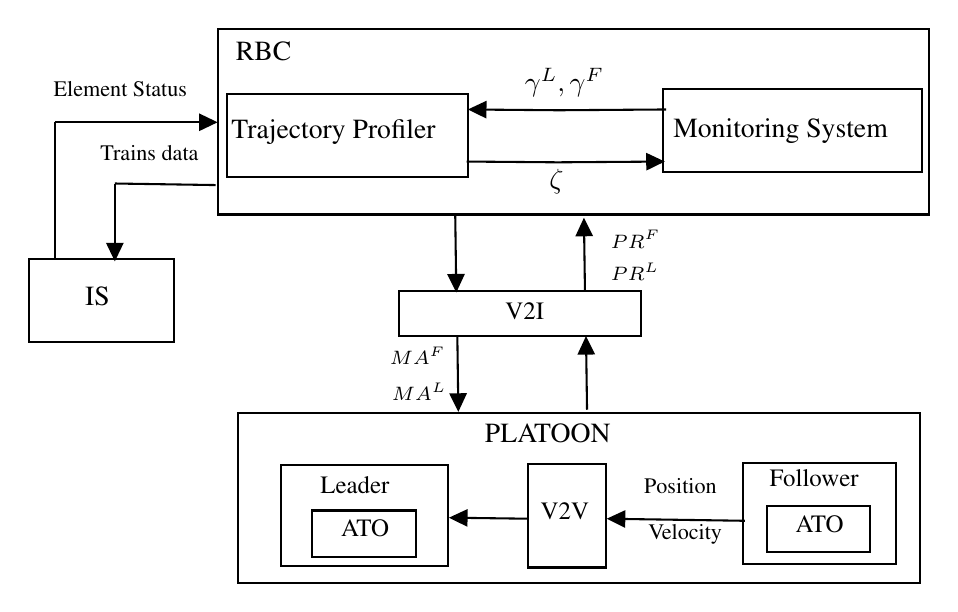
\begin{tikzpicture}[x=0.75pt,y=0.75pt,yscale=-1,xscale=1]
%uncomment if require: \path (0,300); %set diagram left start at 0, and has height of 300

%Shape: Rectangle [id:dp9181587437923022] 
\draw   (172,122.67) -- (242,122.67) -- (242,162.67) -- (172,162.67) -- cycle ;
%Shape: Rectangle [id:dp20903442434187935] 
\draw   (263,11.67) -- (605.67,11.67) -- (605.67,101.17) -- (263,101.17) -- cycle ;
%Shape: Rectangle [id:dp41239476881753845] 
\draw   (273,197) -- (601.5,197) -- (601.5,278.75) -- (273,278.75) -- cycle ;
%Shape: Rectangle [id:dp530653774898959] 
\draw   (267.67,43) -- (383.67,43) -- (383.67,83) -- (267.67,83) -- cycle ;
%Shape: Rectangle [id:dp07362802641529798] 
\draw   (477.56,40.83) -- (602.33,40.83) -- (602.33,80.83) -- (477.56,80.83) -- cycle ;
%Shape: Rectangle [id:dp3493633693136575] 
\draw   (293.5,221.83) -- (374,221.83) -- (374,270.75) -- (293.5,270.75) -- cycle ;
%Shape: Rectangle [id:dp34089559436294614] 
\draw   (350.5,138.25) -- (466.83,138.25) -- (466.83,159.5) -- (350.5,159.5) -- cycle ;
%Shape: Rectangle [id:dp38792726766554986] 
\draw   (412.5,221.25) -- (450,221.25) -- (450,271.25) -- (412.5,271.25) -- cycle ;
%Straight Lines [id:da41264737503221705] 
\draw    (383,75.67) -- (426.84,76.04) -- (475.44,75.69) ;
\draw [shift={(478.44,75.67)}, rotate = 179.58] [fill={rgb, 255:red, 0; green, 0; blue, 0 }  ][line width=0.08]  [draw opacity=0] (8.93,-4.29) -- (0,0) -- (8.93,4.29) -- cycle    ;
%Straight Lines [id:da35026960584329925] 
\draw    (377.5,101.75) -- (377.96,135.75) ;
\draw [shift={(378,138.75)}, rotate = 269.23] [fill={rgb, 255:red, 0; green, 0; blue, 0 }  ][line width=0.08]  [draw opacity=0] (8.93,-4.29) -- (0,0) -- (8.93,4.29) -- cycle    ;
%Straight Lines [id:da16469888193523596] 
\draw    (378.5,159.25) -- (378.96,193.25) ;
\draw [shift={(379,196.25)}, rotate = 269.23] [fill={rgb, 255:red, 0; green, 0; blue, 0 }  ][line width=0.08]  [draw opacity=0] (8.93,-4.29) -- (0,0) -- (8.93,4.29) -- cycle    ;
%Straight Lines [id:da8472970357726008] 
\draw    (440,138.25) -- (439.54,105.75) ;
\draw [shift={(439.5,102.75)}, rotate = 89.19] [fill={rgb, 255:red, 0; green, 0; blue, 0 }  ][line width=0.08]  [draw opacity=0] (8.93,-4.29) -- (0,0) -- (8.93,4.29) -- cycle    ;
%Straight Lines [id:da2638037577347745] 
\draw    (441,195.25) -- (440.54,162.75) ;
\draw [shift={(440.5,159.75)}, rotate = 89.19] [fill={rgb, 255:red, 0; green, 0; blue, 0 }  ][line width=0.08]  [draw opacity=0] (8.93,-4.29) -- (0,0) -- (8.93,4.29) -- cycle    ;
%Shape: Rectangle [id:dp711774726571057] 
\draw   (516.33,220.83) -- (590,220.83) -- (590,269.75) -- (516.33,269.75) -- cycle ;
%Shape: Rectangle [id:dp3073038779813597] 
\draw   (308.5,243.79) -- (358.5,243.79) -- (358.5,266) -- (308.5,266) -- cycle ;
%Shape: Rectangle [id:dp744059415491537] 
\draw   (527.5,241.46) -- (577.5,241.46) -- (577.5,263.67) -- (527.5,263.67) -- cycle ;
%Straight Lines [id:da7367089023216331] 
\draw    (184.5,56.75) -- (260,56.75) ;
\draw [shift={(263,56.75)}, rotate = 180] [fill={rgb, 255:red, 0; green, 0; blue, 0 }  ][line width=0.08]  [draw opacity=0] (8.93,-4.29) -- (0,0) -- (8.93,4.29) -- cycle    ;
%Straight Lines [id:da5062815061117323] 
\draw    (184.5,56.75) -- (184.5,122.75) ;
%Straight Lines [id:da32086022579187445] 
\draw    (213.5,86.25) -- (213.5,120.75) ;
\draw [shift={(213.5,123.75)}, rotate = 270] [fill={rgb, 255:red, 0; green, 0; blue, 0 }  ][line width=0.08]  [draw opacity=0] (8.93,-4.29) -- (0,0) -- (8.93,4.29) -- cycle    ;
%Straight Lines [id:da9349544027263015] 
\draw    (262,87) -- (213.5,86.25) ;
%Straight Lines [id:da8061807028246681] 
\draw    (517,248.75) -- (453.5,247.8) ;
\draw [shift={(450.5,247.75)}, rotate = 0.86] [fill={rgb, 255:red, 0; green, 0; blue, 0 }  ][line width=0.08]  [draw opacity=0] (8.93,-4.29) -- (0,0) -- (8.93,4.29) -- cycle    ;
%Straight Lines [id:da25677830767358123] 
\draw    (412.5,247.75) -- (377.5,247.29) ;
\draw [shift={(374.5,247.25)}, rotate = 0.75] [fill={rgb, 255:red, 0; green, 0; blue, 0 }  ][line width=0.08]  [draw opacity=0] (8.93,-4.29) -- (0,0) -- (8.93,4.29) -- cycle    ;
%Straight Lines [id:da4316689504126945] 
\draw    (386.62,50.61) -- (427.45,50.96) -- (479.06,50.58) ;
\draw [shift={(383.62,50.58)}, rotate = 0.49] [fill={rgb, 255:red, 0; green, 0; blue, 0 }  ][line width=0.08]  [draw opacity=0] (8.93,-4.29) -- (0,0) -- (8.93,4.29) -- cycle    ;

% Text Node
\draw (197.67,134.33) node [anchor=north west][inner sep=0.75pt]   [align=left] {{\fontfamily{ptm}\selectfont IS}};
% Text Node
\draw (270.33,16.17) node [anchor=north west][inner sep=0.75pt]   [align=left] {{\fontfamily{ptm}\selectfont RBC}};
% Text Node
\draw (268.17,53.83) node [anchor=north west][inner sep=0.75pt]   [align=left] {{\fontfamily{ptm}\selectfont Trajectory Profiler}};
% Text Node
\draw (481.06,53.58) node [anchor=north west][inner sep=0.75pt]  [font=\normalsize] [align=left] {{\fontfamily{ptm}\selectfont Monitoring System}};
% Text Node
\draw (400.17,142) node [anchor=north west][inner sep=0.75pt]  [font=\small] [align=left] {{\fontfamily{ptm}\selectfont {\small V2I}}};
% Text Node
\draw (417.17,238.5) node [anchor=north west][inner sep=0.75pt]  [font=\small] [align=left] {{\fontfamily{ptm}\selectfont {\small V2V}}};
% Text Node
\draw (390.33,200.33) node [anchor=north west][inner sep=0.75pt]   [align=left] {{\fontfamily{ptm}\selectfont PLATOON}};
% Text Node
\draw (311,225.83) node [anchor=north west][inner sep=0.75pt]  [font=\small] [align=left] {{\fontfamily{ptm}\selectfont Leader}};
% Text Node
\draw (527.5,222.33) node [anchor=north west][inner sep=0.75pt]  [font=\small] [align=left] {{\fontfamily{ptm}\selectfont Follower}};
% Text Node
\draw (321,246.83) node [anchor=north west][inner sep=0.75pt]  [font=\small] [align=left] {{\small {\fontfamily{ptm}\selectfont ATO}}};
% Text Node
\draw (540,244.5) node [anchor=north west][inner sep=0.75pt]  [font=\small] [align=left] {{\small {\fontfamily{ptm}\selectfont ATO}}};
% Text Node
\draw (345.5,180.9) node [anchor=north west][inner sep=0.75pt]  [font=\scriptsize]  {$MA^{L}$};
% Text Node
\draw (344.5,163.4) node [anchor=north west][inner sep=0.75pt]  [font=\scriptsize]  {$MA^{F}$};
% Text Node
\draw (451,107.4) node [anchor=north west][inner sep=0.75pt]  [font=\scriptsize]  {$PR^{F}$};
% Text Node
\draw (451,122.9) node [anchor=north west][inner sep=0.75pt]  [font=\scriptsize]  {$PR^{L}$};
% Text Node
\draw (467,227) node [anchor=north west][inner sep=0.75pt]   [align=left] {{\fontfamily{ptm}\selectfont {\footnotesize Position}}};
% Text Node
\draw (469,249) node [anchor=north west][inner sep=0.75pt]   [align=left] {{\fontfamily{ptm}\selectfont {\footnotesize Velocity}}};
% Text Node
\draw (205,66.33) node [anchor=north west][inner sep=0.75pt]   [align=left] {{\fontfamily{ptm}\selectfont {\footnotesize Trains data}}};
% Text Node
\draw (182.5,35.5) node [anchor=north west][inner sep=0.75pt]  [font=\normalsize] [align=left] {{\footnotesize {\fontfamily{ptm}\selectfont Element Status}}};
% Text Node
\draw (421.33,77.73) node [anchor=north west][inner sep=0.75pt]    {$\zeta $};
% Text Node
\draw (409.58,29.26) node [anchor=north west][inner sep=0.75pt]    {$\gamma ^{L} ,\gamma ^{F}$};


\end{tikzpicture}

